\documentclass[journal,12pt,twocolumn]{IEEEtran}

\usepackage{setspace}
\usepackage{gensymb}
\singlespacing
\usepackage[cmex10]{amsmath}

\usepackage{amsthm}

\usepackage{mathrsfs}
\usepackage{txfonts}
\usepackage{stfloats}
\usepackage{bm}
\usepackage{cite}
\usepackage{cases}
\usepackage{subfig}

\usepackage{longtable}
\usepackage{multirow}

\usepackage{enumitem}
\usepackage{mathtools}
\usepackage{steinmetz}
\usepackage{tikz}
\usepackage{circuitikz}
\usepackage{verbatim}
\usepackage{tfrupee}
\usepackage[breaklinks=true]{hyperref}
\usepackage{graphicx}
\usepackage{tkz-euclide}

\usetikzlibrary{calc,math}
\usepackage{listings}
    \usepackage{color}                                            %%
    \usepackage{array}                                            %%
    \usepackage{longtable}                                        %%
    \usepackage{calc}                                             %%
    \usepackage{multirow}                                         %%
    \usepackage{hhline}                                           %%
    \usepackage{ifthen}                                           %%
    \usepackage{lscape}     
\usepackage{multicol}
\usepackage{chngcntr}

\DeclareMathOperator*{\Res}{Res}

\renewcommand\thesection{\arabic{section}}
\renewcommand\thesubsection{\thesection.\arabic{subsection}}
\renewcommand\thesubsubsection{\thesubsection.\arabic{subsubsection}}

\renewcommand\thesectiondis{\arabic{section}}
\renewcommand\thesubsectiondis{\thesectiondis.\arabic{subsection}}
\renewcommand\thesubsubsectiondis{\thesubsectiondis.\arabic{subsubsection}}


\hyphenation{op-tical net-works semi-conduc-tor}
\def\inputGnumericTable{}                                 %%

\lstset{
%language=C,
frame=single, 
breaklines=true,
columns=fullflexible
}
\begin{document}


\newtheorem{theorem}{Theorem}[section]
\newtheorem{problem}{Problem}
\newtheorem{proposition}{Proposition}[section]
\newtheorem{lemma}{Lemma}[section]
\newtheorem{corollary}[theorem]{Corollary}
\newtheorem{example}{Example}[section]
\newtheorem{definition}[problem]{Definition}

\newcommand{\BEQA}{\begin{eqnarray}}
\newcommand{\EEQA}{\end{eqnarray}}
\newcommand{\define}{\stackrel{\triangle}{=}}
\bibliographystyle{IEEEtran}
\raggedbottom
\setlength{\parindent}{0pt}
\providecommand{\mbf}{\mathbf}
\providecommand{\pr}[1]{\ensuremath{\Pr\left(#1\right)}}
\providecommand{\qfunc}[1]{\ensuremath{Q\left(#1\right)}}
\providecommand{\sbrak}[1]{\ensuremath{{}\left[#1\right]}}
\providecommand{\lsbrak}[1]{\ensuremath{{}\left[#1\right.}}
\providecommand{\rsbrak}[1]{\ensuremath{{}\left.#1\right]}}
\providecommand{\brak}[1]{\ensuremath{\left(#1\right)}}
\providecommand{\lbrak}[1]{\ensuremath{\left(#1\right.}}
\providecommand{\rbrak}[1]{\ensuremath{\left.#1\right)}}
\providecommand{\cbrak}[1]{\ensuremath{\left\{#1\right\}}}
\providecommand{\lcbrak}[1]{\ensuremath{\left\{#1\right.}}
\providecommand{\rcbrak}[1]{\ensuremath{\left.#1\right\}}}
\theoremstyle{remark}
\newtheorem{rem}{Remark}
\newcommand{\sgn}{\mathop{\mathrm{sgn}}}
\providecommand{\res}[1]{\Res\displaylimits_{#1}} 
%\providecommand{\norm}[1]{\lVert#1\rVert}
\providecommand{\mtx}[1]{\mathbf{#1}}
\providecommand{\fourier}{\overset{\mathcal{F}}{ \rightleftharpoons}}
%\providecommand{\hilbert}{\overset{\mathcal{H}}{ \rightleftharpoons}}
\providecommand{\system}{\overset{\mathcal{H}}{ \longleftrightarrow}}
	%\newcommand{\solution}[2]{\textbf{Solution:}{#1}}
\newcommand{\solution}{\noindent \textbf{Solution: }}
\newcommand{\cosec}{\,\text{cosec}\,}
\providecommand{\dec}[2]{\ensuremath{\overset{#1}{\underset{#2}{\gtrless}}}}
\newcommand{\myvec}[1]{\ensuremath{\begin{pmatrix}#1\end{pmatrix}}}
\newcommand{\mydet}[1]{\ensuremath{\begin{vmatrix}#1\end{vmatrix}}}
\numberwithin{equation}{subsection}
\makeatletter
\@addtoreset{figure}{problem}
\makeatother
\let\StandardTheFigure\thefigure
\let\vec\mathbf
\renewcommand{\thefigure}{\theproblem}
\def\putbox#1#2#3{\makebox[0in][l]{\makebox[#1][l]{}\raisebox{\baselineskip}[0in][0in]{\raisebox{#2}[0in][0in]{#3}}}}
     \def\rightbox#1{\makebox[0in][r]{#1}}
     \def\centbox#1{\makebox[0in]{#1}}
     \def\topbox#1{\raisebox{-\baselineskip}[0in][0in]{#1}}
     \def\midbox#1{\raisebox{-0.5\baselineskip}[0in][0in]{#1}}
\vspace{3cm}
\title{EE3025 IDP Assignment-1}
\author{C.SriRam Saran-EE18BTECH11007}
\maketitle
\newpage
\bigskip
\renewcommand{\thefigure}{\theenumi}
\renewcommand{\thetable}{\theenumi}
Download all python codes from 
\begin{lstlisting}
https://github.com/csrs2000/EE3025_IDP/tree/main/Assignment-1/code
\end{lstlisting}
%
and latex-tikz codes from 
%
\begin{lstlisting}
https://github.com/csrs2000/EE3025_IDP/tree/main/Assignment-1
\end{lstlisting}
\section{Question}
\begin{enumerate}[label=\thesection.\arabic*.,ref=\thesection.\theenumi]
\numberwithin{equation}{enumi}
    
\item Let
\begin{align}
    x(n) = \cbrak{\underset{\uparrow}{1},2,3,4,2,1} \\
    y(n) + \frac{1}{2}y(n-1) = x(n) + x(n-2) \label{eq:1.0.2}
\end{align}
Compute
\begin{align}
    X(k) \triangleq \sum_{n=0}^{N-1}x(n)e^{-j2\pi kn/N},\quad k=0,1, \ldots, N-1
\end{align}
and $H(k)$ using $h(n)$.
\end{enumerate}
\section{Solution}
\begin{enumerate}[label=\thesection.\arabic*.,ref=\thesection.\theenumi]
\numberwithin{equation}{enumi}
\item
When Unit impulse signal is given as input to the LTI system then its impulse response is the ouput of the system.
So,from equation \eqref{eq:1.0.2} we can say that the Impulse response of the system is,
\begin{align}
    h(n) + \frac{1}{2}h(n-1) = \delta(n) + \delta(n-2)	
\end{align}
\item DFT of a Input Signal $x(n)$ is :
\begin{align}
    X(k) \triangleq \sum_{n=0}^{N-1}x(n)e^{-j2\pi kn/N},\quad k=0,1, \ldots, N-1 \label{eq:2.0.2}
\end{align}
Similarly, DFT of Impulse Response $h(n)$ is,
\begin{align}
    H(k) \triangleq \sum_{n=0}^{N-1}h(n)e^{-j2\pi kn/N},\quad k=0,1, \ldots, N-1 \label{eq:2.0.3}
\end{align}
\item
Dft matrix multiplication method- DFT of x(n) and h(n) using Matrix multiplication method
\\
\begin{align}
    X(k) \triangleq \sum_{n=0}^{N-1}x(n)e^{-j2\pi kn/N},\quad k=0,1, \ldots, N-1
\end{align}
Lets take $W_N^{nk}=e^{-j2\pi kn/N} $,
expressing $X(k)$ in terms of product of DFT matrix and $x(k)$:
\begin{equation}
 \begin{bmatrix} X(0) \\ X(1) \\ X(2) \\ X(3) \\ X(4) \\ X(5) \end{bmatrix}
=
\begin{bmatrix}
1 & 1 & 1 & 1 & 1 & 1 \\ 1 & W_N^1& W_N^2& W_N^3 & W_N^4 & W_N^5\\1 & W_N^2 & W_N^4 & W_N^6 & W_N^8 & W_N^{10}\\1 & W_N^3 & W_N^6 & W_N^9 & W_N^{12} & W_N^{15}\\1 & W_N^4 & W_N^8 & W_N^{12} & W_N^{16} & W_N^{20}\\1 & W_N^5 & W_N^{10} & W_N^{15} & W_N^{20} &W_N^{25}
\end{bmatrix}%
\begin{bmatrix}
x(0) \\ x(1) \\ x(2) \\ x(3) \\ x(4) \\x(5)
\end{bmatrix}
\end{equation}
given x(n) = \cbrak{\underset{\uparrow}{1},2,3,4,2,1} \\,here N=6 so above equation becomes
\begin{equation}
\begin{bmatrix} X(0) \\ X(1) \\ X(2) \\ X(3) \\ X(4) \\ X(5) \end{bmatrix}
=
\begin{bmatrix}
1 +2+3+4+2+1 \\ 1+ (2)e^{-j\pi /3} + ... + (1)e^{-j5\pi /3}\\ 1 + (2)e^{-2j\pi /3} + ... +(1)(e^{-2j5\pi /3}\\ 1 + (2)e^{-3j\pi /3} + ... + (1)e^{-3j5\pi /3}\\ 1 + (2)e^{-4j\pi /3} + ... + (1)e^{-4j5\pi /3}\\ 1 + (2)e^{-5j\pi /3} + ... + (1)e^{-5j5\pi /3}
\end{bmatrix}
\end{equation}
\
On solving we get,
\begin{align}
    \implies X(0) = 13 + 0j,\\
    X(1) = -4 - 1.732j,\\
    X(2) = 1 + 0j,
    \\
    X(3) = -1 + 0j,\\
    X(4) = 1 + 0j,\\
    X(5) = -4 + 1.732j
\end{align}
in order to find $H(k)$ we need to find h(n) first. So we will first calculate h(n). we will find that using Y(Z),X(Z)For that we need to first find the Y(z) by applying Z-transform on equation $\eqref{eq:1.0.2}$ i.e.,
\begin{align}
    Y(z) + \frac{1}{2}z^{-1}Y(z)=X(z) + z^{-2}X(z)
\end{align}
\begin{align}
    \implies Y(z)=\frac{2(z^2+1)}{z(2z+1)}X(z)
\end{align}
\
Now we can find H(z) using Y(z)\\
 i.e.,
\begin{align}
    H(z) = \frac{Y(z)}{X(z)}
\end{align}
\begin{align}
 H(z) = \frac{2(z^2+1)}{z(2z+1)}
\end{align}
\begin{align}
 H(z) = \frac{1+z^{-2}}{1+\frac{1}{2}z^{-1}}
\end{align}
 h(n) is,
\begin{align}
 H(Z)= Z^{-1}\sbrak{\frac{1}{1+\frac{1}{2}z^{-1}} + \frac{z^{-2}}{1+\frac{1}{2}z^{-1}}}
\end{align}
\begin{align}
 h(n)=\sbrak{\frac{-1}{2}}^nu(n) + \sbrak{\frac{-1}{2}}^{n-2}u(n-2)
\end{align}
\
\
lets  assume that length of h(n) is 6,i.e, N = 6.
using matrix multiplication method we obtain
\begin{equation}
\begin{bmatrix} H(0) \\ H(1) \\ H(2) \\ H(3) \\ H(4) \\ H(5) \end{bmatrix}
=
\begin{bmatrix}
 h(0)+..+h(5)\\h(0)+h(1)e^{-j\pi/3}+..+h(5)e^{-j5\pi/3}\\h(0)+h(1)e^{-2j\pi/3}+..+h(5)e^{-2j5\pi/3}\\h(0)+h(1)e^{-3j\pi /3}+..+h(5)e^{-3j5\pi/3}\\h(0)+h(1)e^{-4j\pi /3}+...+h(5)e^{-4j5\pi/3}\\h(0)+h(1)e^{-5j\pi/3}+..+h(5)e^{-5j5\pi/3}
\end{bmatrix}
\end{equation}
On calculating we get,
\begin{align}
\implies H(0) = 1.28125 + 0j,\\
 H(1) = 0.51625 - 0.5141875j,\\
 H(2) = -0.078125 + 1.1095625j,\\
 H(3) = 3.84375 + 0j,\\
 H(4) = -0.071825 - 1.1095625j.\\
 H(5) = 0.515625 + 0.5141875j
\end{align}
lets verify these values by using python code
\\
\\
\\
\item Python Code to compute the DFT of $x(n)$ and $h(n)$ is given below
\begin{lstlisting}
https://github.com/csrs2000/EE3025_IDP/blob/main/Assignment-1/code/ee18btech11007.py
\end{lstlisting}
\item using the above code we get the following plots.
\begin{lstlisting}
https://github.com/csrs2000/EE3025_IDP/tree/main/Assignment-1/figs
\end{lstlisting}
\begin{figure}[h!]
    \centering
    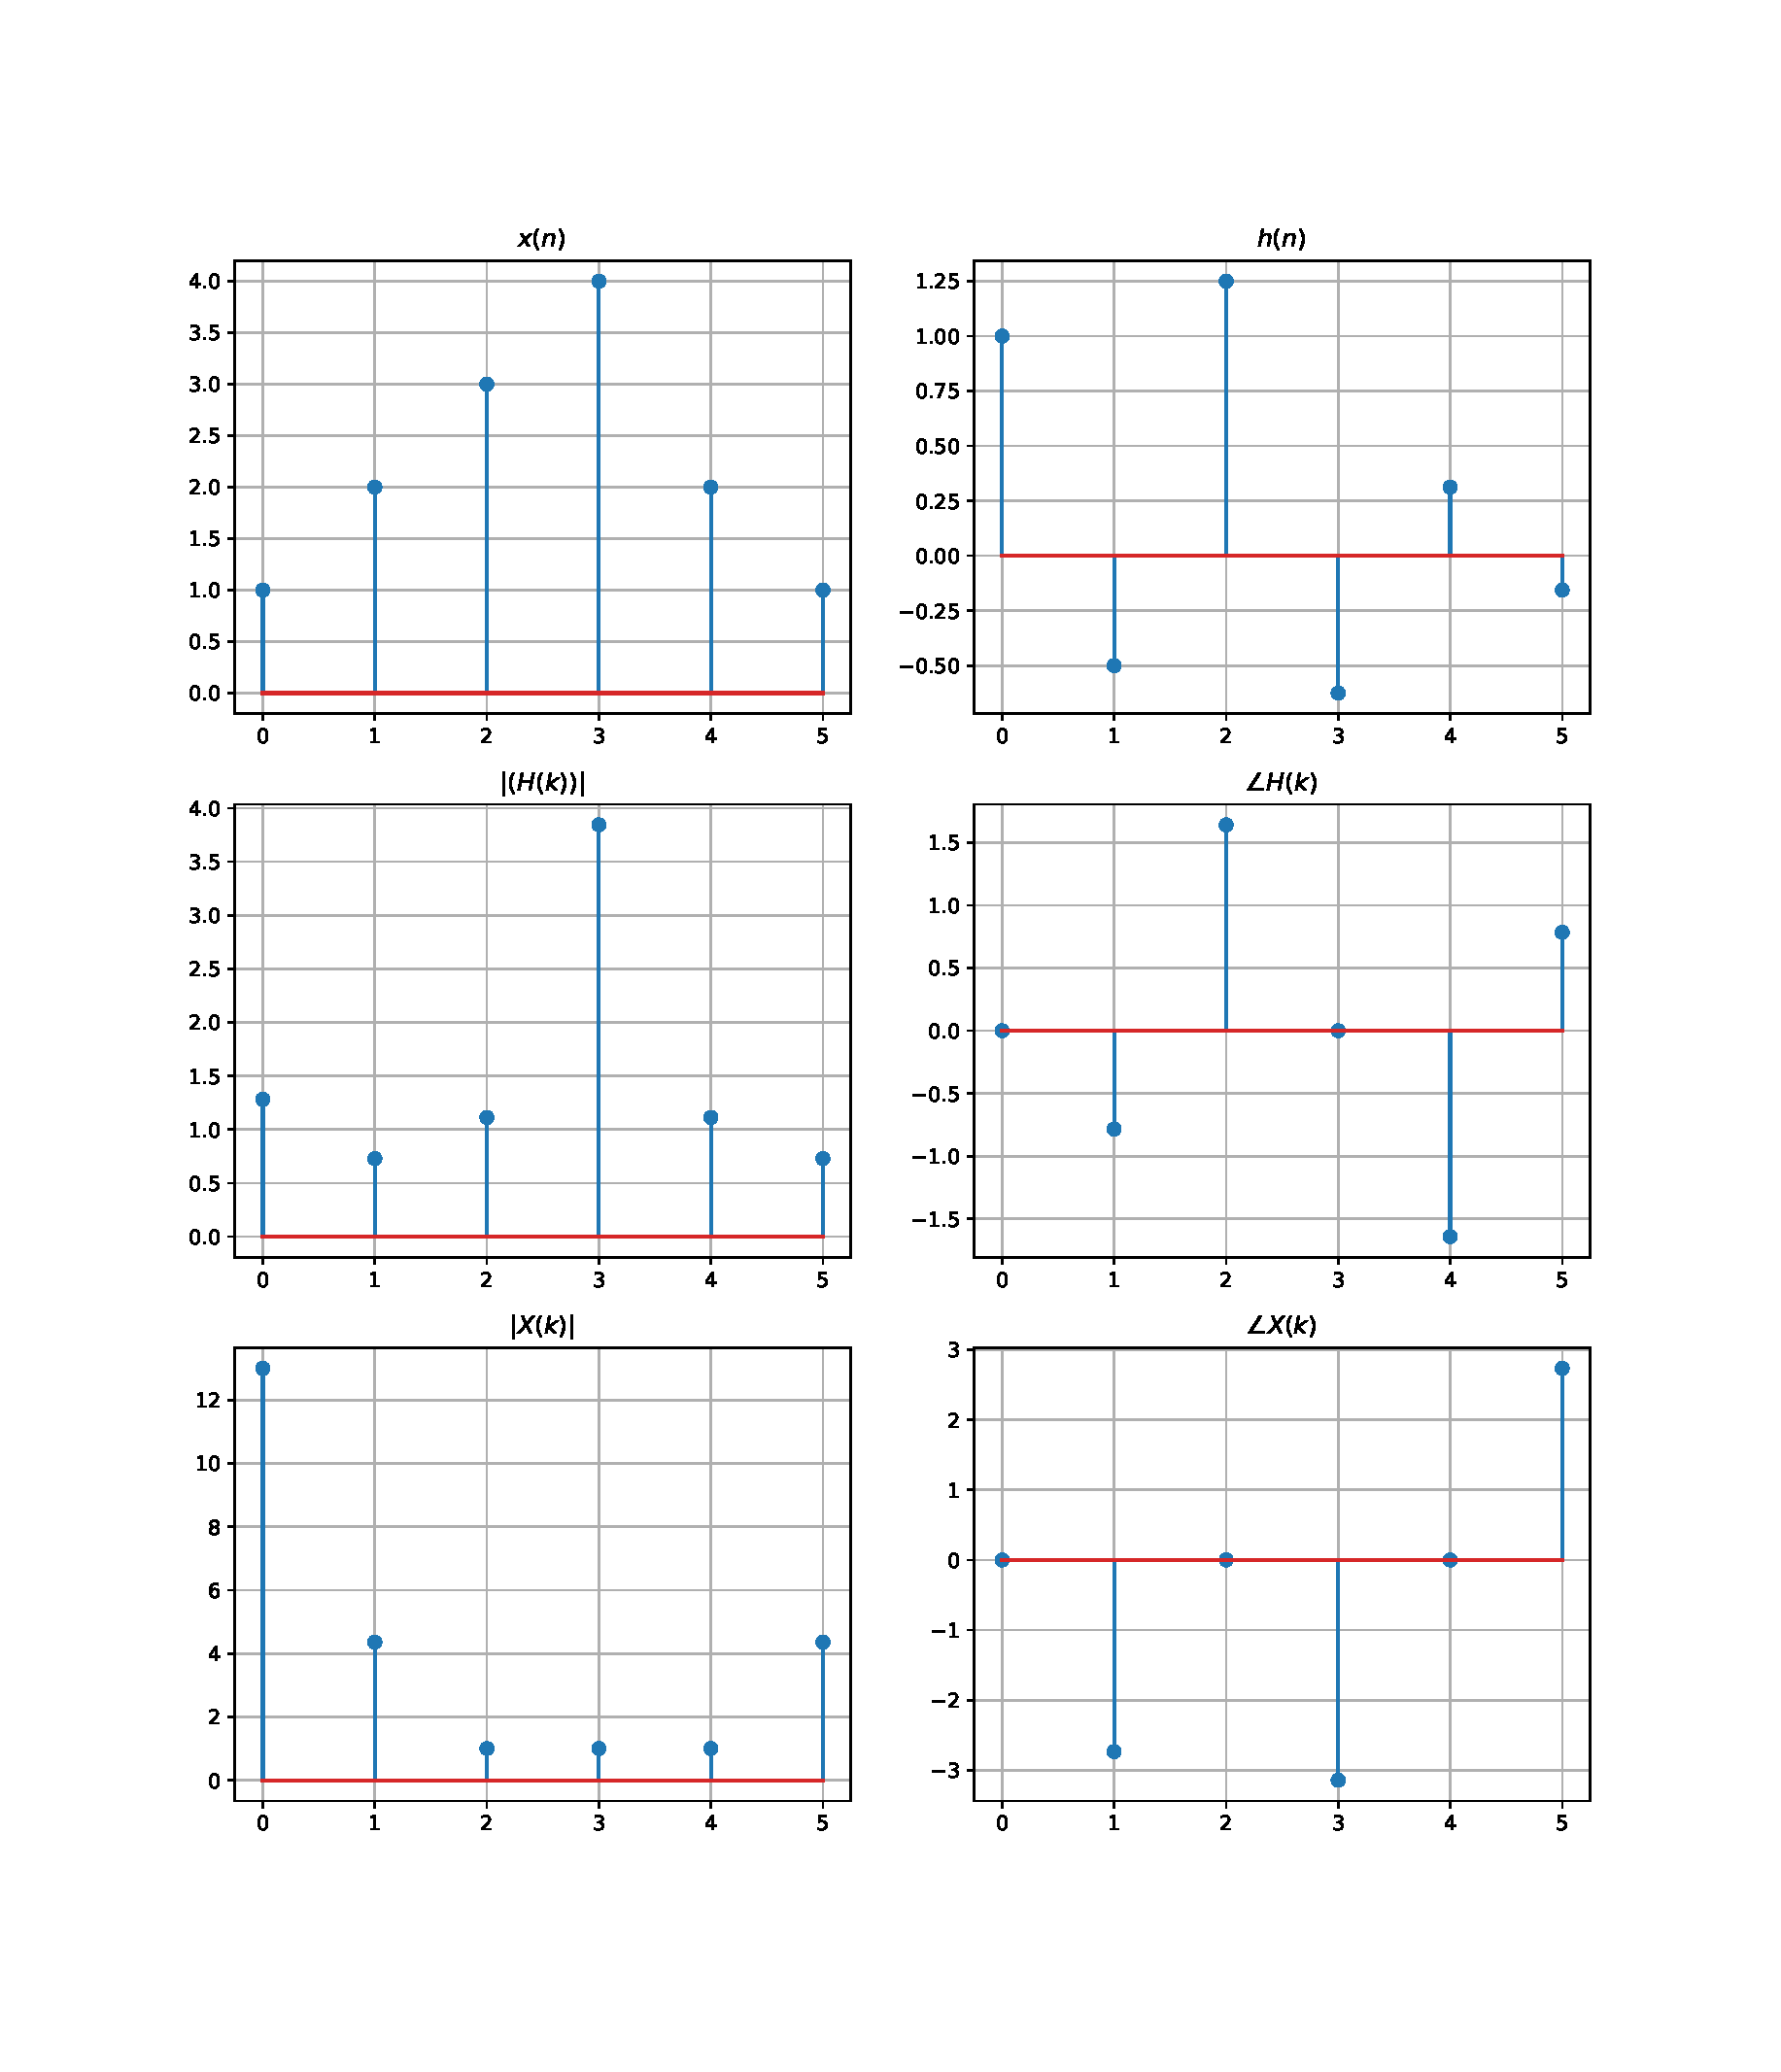
\includegraphics[width=10cm]{./figs/ee18btech11007.eps}
    \caption{Plots of x(n) and h(n),their DFTs}
    \label{figs}
\end{figure}
manually calculated values match with the values obtained from codes
\end{enumerate}

\section{Approach-2}
\begin{enumerate}[label=\thesection.\arabic*.,ref=\thesection.\theenumi]
\numberwithin{equation}{enumi}
\item \emph{Properties of $W_{N}$}
\begin{enumerate}
\item Property-1 : \[ W^{2}_{N} =  W_{N/2} \]  
\item Property-2 : \[ W^{k+N/2}_{N} = - W^{k}_{N} \]
\end{enumerate}
\item  a N-point DFT is computed as,
    \begin{align}
        X(k) = \sum_{n=0}^{N-1} x(n)W^{nk}_{N}, \quad k=0,1, \ldots, N-1
    \end{align}
now for easier calculations we can Divide the inputs into even and odd indices and using Property-1,
    \begin{align}
       X(k) &= \sum_{n=even} x(n)W^{kn}_{N} + \sum_{n=odd} x(n)W^{kn}_{N} \\
       &= \sum_{m=0}^{N/2 -1} x(2m)W^{2mk}_{N} + \sum_{m=0}^{N/2 -1} x(2m+1)W^{(2m+1)k}_{N} \\
       &= \sum_{m=0}^{N/2 -1} x(2m)W^{mk}_{N/2} + W^{k}_{N} \sum_{m=0}^{N/2 -1} x(2m+1)W^{mk}_{N/2} 
    \end{align}
by observing,
\begin{align}
X(k) = {X_{e}(k)}+ W_{N}^k{X_{o}(k)}
\label{eq:equation3}
\end{align}

    
for the given question  N = 6, we can express the even odd DFT's $X_{e}(k)$ , $X_{o}(k)$ interms of block  matrices, we obtain,
\begin{equation}
\begin{bmatrix}
X_{e}(0) \\ 
X_{e}(1) \\ 
X_{e}(2) \\ 
X_{o}(0) \\ 
X_{o}(1) \\ 
X_{o}(2)
\end{bmatrix}
=
\begin{bmatrix}
W^{0}_{3} & W^{0}_{3} & W^{0}_{3} & 0 & 0 & 0\\
W^{0}_{3} & W^{1}_{3} & W^{2}_{3} & 0 & 0 & 0\\
W^{0}_{3} & W^{2}_{3} & W^{4}_{3} & 0 & 0 & 0\\
0 & 0 & 0 & W^{0}_{3} & W^{0}_{3} & W^{0}_{3}\\
0 & 0 & 0 & W^{0}_{3} & W^{1}_{3} & W^{2}_{3}\\
0 & 0 & 0 & W^{0}_{3} & W^{2}_{3} & W^{4}_{3}
\end{bmatrix}
\begin{bmatrix}
x(0) \\ 
x(2) \\ 
x(4) \\ 
x(1) \\ 
x(3) \\ 
x(5) 
\end{bmatrix}   
\end{equation}
    
Lets take , $F_{N}$ as a N-Point DFT Matrix and $P_{N}$ as an odd-even Permutation Matrix, we can write above equation as
\begin{equation}
\begin{bmatrix}
X_{e}(0) \\ 
X_{e}(1) \\ 
X_{e}(2) \\ 
X_{o}(0) \\ 
X_{o}(1) \\ 
X_{o}(2)
\end{bmatrix}
=
\begin{bmatrix}
F_{3} & 0 \\
0 & F_{3}
\end{bmatrix}
P_{6}
x   
\label{eq:equation6}
\end{equation}
where
\begin{equation}
P_{6} 
=
\begin{bmatrix}
1 & 0 & 0 & 0 & 0 & 0\\
0 & 0 & 1 & 0 & 0 & 0\\
0 & 0 & 0 & 0 & 1 & 0\\
0 & 1 & 0 & 0 & 0 & 0\\
0 & 0 & 0 & 1 & 0 & 0\\
0 & 0 & 0 & 0 & 0 & 1
\end{bmatrix} 
\end{equation}
and 
\begin{equation}
P_{6}x
=
P_{6}
\begin{bmatrix}
x(0) \\ 
x(1) \\ 
x(2) \\ 
x(3) \\ 
x(4) \\ 
x(5) 
\end{bmatrix}
=
\begin{bmatrix}
x(0) \\ 
x(2) \\ 
x(4) \\ 
x(1) \\ 
x(3) \\ 
x(5) 
\end{bmatrix}   
\end{equation}
Now,using \eqref{eq:equation3} we can formulate  $X(k)$ interms of $X_{e}(k)$ and $X_{o}(k)$
\begin{equation}
\begin{bmatrix}
X(0) \\ 
X(1) \\ 
X(2) \\ 
X(3) \\ 
X(4) \\ 
X(5) 
\end{bmatrix}
=
\begin{bmatrix}
1 & 0 & 0 & W^{0}_{6} & 0 & 0\\
0 & 1 & 0 &  0 & W^{1}_{6} & 0\\
0 & 0 & 1 & 0 & 0 & W^{2}_{6}\\
1 & 0 & 0 & W^{3}_{6} & 0 & 0\\
0 & 1 & 0 & 0 & W^{4}_{6} & 0\\
0 & 0 & 1 & 0 & 0 & W^{5}_{6}
\end{bmatrix}
\begin{bmatrix}
X_{e}(0) \\ 
X_{e}(1) \\ 
X_{e}(2) \\ 
X_{o}(0) \\ 
X_{o}(1) \\ 
X_{o}(2)
\end{bmatrix}
\label{eq:equation4}
\end{equation}
lets assume  $I_{3}$ to be 3x3 identity matrix and $D_{N} = diag(1,W_{N},W_{N}^{2},....,W_{N}^{N-1})$ .accordingly we get  $D_{\frac{N}{2}} = diag(1,W_{N},W_{N}^{2},....,W_{N}^{\frac{N}{2} -1})$.so  $D_{3}$ will be,
\begin{equation}
D_{3}=
\begin{bmatrix}
1 & 0 & 0 \\
0 & W^{1}_{6} & 0 \\
0 & 0 & W^{2}_{6}
\end{bmatrix}
\end{equation}
Using Property-2, Equation \eqref{eq:equation4} gets expressed  in terms of   $D_{3}$ and $I_{3}$ as,
\begin{equation}
X
=
\begin{bmatrix}
X(0) \\ 
X(1) \\ 
X(2) \\ 
X(3) \\ 
X(4) \\ 
X(5) 
\end{bmatrix}
=
\begin{bmatrix}
I_{3} & D_{3} \\
I_{3} & -D_{3}
\end{bmatrix}
\begin{bmatrix}
X_{e}(0) \\ 
X_{e}(1) \\ 
X_{e}(2) \\ 
X_{o}(0) \\ 
X_{o}(1) \\ 
X_{o}(2)
\end{bmatrix}
\label{eq:equation5}
\end{equation}
Finally using Eq \eqref{eq:equation5} and Eq \eqref{eq:equation6} we obtain
\begin{equation}
X
=
\begin{bmatrix}
I_{3} & D_{3} \\
I_{3} & -D_{3}
\end{bmatrix}
\begin{bmatrix}
F_{3} & 0 \\
0 & F_{3}
\end{bmatrix}
P_{6}
x 
\label{eq:equation7}
\end{equation}
we know  $X = F_{6}x$ for N = 6 hence we obtain $F_{6}$ as ;
\begin{equation}
\implies 
F_{6}
=
\begin{bmatrix}
I_{3} & D_{3} \\
I_{3} & -D_{3}
\end{bmatrix}
\begin{bmatrix}
F_{3} & 0 \\
0 & F_{3}
\end{bmatrix}
P_{6}
\end{equation}
above approach can be used for any  arbitary $N$ , lets take a N-point DFT Matrix and express it  in terms of N/2-point DFT Matrix as
\begin{equation} 
F_{N}
=
\begin{bmatrix}
I_{N/2} & D_{N/2} \\
I_{N/2} & -D_{N/2}
\end{bmatrix}
\begin{bmatrix}
F_{N/2} & 0 \\
0 & F_{N/2}
\end{bmatrix}
P_{N}
\label{eq:equation8}
\end{equation}
\item Now,for any  $N = 2^{m}$ where $m \in \mathbb{Z^{+}}$  we can recursively breakdown N/2 point DFT Matrix to N/4 point DFT Matrix ..so on untill we reach 2-point DFT Matrix.for N = 8, we can break it down using Eq \eqref{eq:equation8} as follows,
\begin{equation}
F_{8}=
\begin{bmatrix}
I_{4} & D_{4} \\
I_{4} & -D_{4}
\end{bmatrix}
\begin{bmatrix}
F_{4} & 0 \\
0 & F_{4}
\end{bmatrix}
P_{8}
\end{equation}
\begin{equation}
F_{4}=
\begin{bmatrix}
I_{2} & D_{2} \\
I_{2} & -D_{2}
\end{bmatrix}
\begin{bmatrix}
F_{2} & 0 \\
0 & F_{2}
\end{bmatrix}
P_{4}
\end{equation}
Finally,we reach  the 2-point DFT Matrix base case 
\begin{equation}
F_{2}
\begin{bmatrix}
x_{1} \\
x_{2}
\end{bmatrix}
=
\begin{bmatrix}
1 & 1 \\
1 & -1
\end{bmatrix}
\begin{bmatrix}
x_{1} \\
x_{2}
\end{bmatrix}
=
\begin{bmatrix}
x_{1}+x_{2} \\
x_{1}-x_{2}
\end{bmatrix}
\end{equation}
\item lets compute the 8-point dft using Step by Step visualization of recursion.
\begin{equation}
\begin{bmatrix}
X(0) \\ 
X(1) \\ 
X(2) \\ 
X(3)
\end{bmatrix}
=
\begin{bmatrix}
X_{e}(0) \\ 
X_{e}(1)\\ 
X_{e}(2)\\
X_{e}(3)\\
\end{bmatrix}
+
\begin{bmatrix}
W^{0}_{8} & 0 & 0 & 0\\
0 & W^{1}_{8} & 0 & 0\\
0 & 0 & W^{2}_{8} & 0\\
0 & 0 & 0 & W^{3}_{8}
\end{bmatrix}
\begin{bmatrix}
X_{o}(0) \\ 
X_{o}(1) \\ 
X_{o}(2) \\
X_{o}(3)
\end{bmatrix}
\end{equation}
\begin{equation}
\begin{bmatrix}
X(4) \\ 
X(5) \\ 
X(6) \\ 
X(7)
\end{bmatrix}
=
\begin{bmatrix}
X_{e}(0) \\ 
X_{e}(1)\\ 
X_{e}(2)\\
X_{e}(3)\\
\end{bmatrix}
-
\begin{bmatrix}
W^{0}_{8} & 0 & 0 & 0\\
0 & W^{1}_{8} & 0 & 0\\
0 & 0 & W^{2}_{8} & 0\\
0 & 0 & 0 & W^{3}_{8}
\end{bmatrix}
\begin{bmatrix}
X_{o}(0) \\ 
X_{o}(1) \\ 
X_{o}(2) \\
X_{o}(3)
\end{bmatrix}
\end{equation}
Now, 4-point DFT's to 2-point DFT's
\begin{equation}
\begin{bmatrix}
X_{e}(0) \\ 
X_{e}(1)\\ 
\end{bmatrix}
=
\begin{bmatrix}
X_{e_{1}}(0) \\ 
X_{e_{1}}(1)\\ 
\end{bmatrix}
+
\begin{bmatrix}
W^{0}_{4} & 0\\
0 & W^{1}_{4}
\end{bmatrix}
\begin{bmatrix}
X_{o_{1}}(0) \\ 
X_{o_{1}}(1) \\ 
\end{bmatrix}
\end{equation}
\begin{equation}
\begin{bmatrix}
X_{e}(2) \\ 
X_{e}(3)\\ 
\end{bmatrix}
=
\begin{bmatrix}
X_{e_{1}}(0) \\ 
X_{e_{1}}(1)\\ 
\end{bmatrix}
-
\begin{bmatrix}
W^{0}_{4} & 0\\
0 & W^{1}_{4}
\end{bmatrix}
\begin{bmatrix}
X_{o_{1}}(0) \\ 
X_{o_{1}}(1) \\ 
\end{bmatrix}
\end{equation}
\begin{equation}
\begin{bmatrix}
X_{o}(0) \\ 
X_{o}(1)\\ 
\end{bmatrix}
=
\begin{bmatrix}
X_{e_{2}}(0) \\ 
X_{e_{2}}(1)\\ 
\end{bmatrix}
+
\begin{bmatrix}
W^{0}_{4} & 0\\
0 & W^{1}_{4}
\end{bmatrix}
\begin{bmatrix}
X_{o_{2}}(0) \\ 
X_{o_{2}}(1) \\ 
\end{bmatrix}
\end{equation}
\begin{equation}
\begin{bmatrix}
X_{o}(2) \\ 
X_{o}(3)\\ 
\end{bmatrix}
=
\begin{bmatrix}
X_{e_{2}}(0) \\ 
X_{e_{2}}(1)\\ 
\end{bmatrix}
-
\begin{bmatrix}
W^{0}_{4} & 0\\
0 & W^{1}_{4}
\end{bmatrix}
\begin{bmatrix}
X_{o_{2}}(0) \\ 
X_{o_{2}}(1) \\ 
\end{bmatrix}
\end{equation}
\begin{equation}
P_{8}
\begin{bmatrix}
x(0) \\ 
x(1) \\ 
x(2) \\ 
x(3) \\ 
x(4) \\ 
x(5) \\
x(6) \\
x(7)
\end{bmatrix}
 = 
\begin{bmatrix}
x(0) \\ 
x(2) \\ 
x(4) \\ 
x(6) \\
x(1) \\ 
x(3) \\ 
x(5) \\
x(7)
\end{bmatrix}
\end{equation}
\begin{equation}
P_{4}
\begin{bmatrix}
x(0) \\ 
x(2) \\ 
x(4) \\ 
x(6) \\
\end{bmatrix}
 = 
\begin{bmatrix}
x(0) \\ 
x(4) \\ 
x(2) \\
x(6)
\end{bmatrix}
\end{equation}
\begin{equation}
P_{4}
\begin{bmatrix}
x(1) \\ 
x(3) \\ 
x(5) \\
x(7)
\end{bmatrix}
 = 
\begin{bmatrix}
x(1) \\ 
x(5) \\ 
x(3) \\ 
x(7) \\
\end{bmatrix}
\end{equation}
at last we get,
\begin{equation}
\begin{bmatrix}
X_{e_{1}}(0) \\ 
X_{e_{1}}(1)\\ 
\end{bmatrix}
= F_{2}
\begin{bmatrix}
x(0) \\ 
x(4) \\ 
\end{bmatrix}
=
\begin{bmatrix}
x(0)+x(4) \\ 
x(0)-x(4) \\ 
\end{bmatrix}
\end{equation}
\begin{equation}
\begin{bmatrix}
X_{o_{1}}(0) \\ 
X_{o_{1}}(1)\\ 
\end{bmatrix}
= F_{2}
\begin{bmatrix}
x(2) \\ 
x(6) \\ 
\end{bmatrix}
=
\begin{bmatrix}
x(2)+x(6) \\ 
x(2)-x(6) \\ 
\end{bmatrix}
\end{equation}
\begin{equation}
\begin{bmatrix}
X_{e_{2}}(0) \\ 
X_{e_{2}}(1)\\ 
\end{bmatrix}
= F_{2}
\begin{bmatrix}
x(1) \\ 
x(5) \\ 
\end{bmatrix}
=
\begin{bmatrix}
x(1)+x(5) \\ 
x(1)-x(5) \\ 
\end{bmatrix}
\end{equation}
\begin{equation}
\begin{bmatrix}
X_{o_{2}}(0) \\ 
X_{o_{2}}(1)\\ 
\end{bmatrix}
= F_{2}
\begin{bmatrix}
x(3) \\ 
x(7) \\ 
\end{bmatrix}
=
\begin{bmatrix}
x(3)+x(7) \\ 
x(3)-x(7) \\ 
\end{bmatrix}
\end{equation}
So, $X_{e_{2}} \in \text{DFT} \{x(1),x(5)\}$ and $X_{o_{2}} \in \text{DFT} \{x(3),x(7)\}$ would combine to give $X_{o}$ .And $X_{e_{1}} \in \text{DFT} \{x(0),x(4)\}$ and $X_{o_{1}} \in \text{DFT} \{x(2),x(6)\}$ would combine to give $X_{e}$.
\item \emph{Time Complexity:} \\
In DFT we perform  Matrix multiplication of NxN matrix with Nx1 vector.
Hence it has $O(N^2)$ time complexity which is very tedious and slow for high values of  $N$.
\newline
the recursion relation for for the above example can be formulated as below recursion tree
\begin{equation}
    T(n) = 2T(n/2) + O(n)
\end{equation}
by Solving above recurrence relation the time complexity is obtained as $O(NlogN)$ which is much faster than $O(N^2)$ for high values of N we can analyse this by plotting in python.

\item The following code plots time complexity of fft,dft
\begin{lstlisting}
https://github.com/csrs2000/EE3025_IDP/blob/main/Assignment-1/code/ee18btech11007_2.py
\end{lstlisting}

\item Computing $X(k)$, $H(k)$ and $Y(k)$ for 
    \begin{align}
        x(n) = \cbrak{\underset{\uparrow}{1},2,3,4,2,1,0,0}
    \end{align}
with N = 8, using above FFT approach.
\begin{figure}[!ht]
	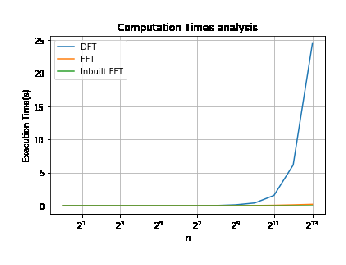
\includegraphics[width=1.15\columnwidth]{./figs/ee18btech11007_2.eps}
\end{figure}
We can observe that both the approaches produces that same plots.
\item The following code plots magnitude and phase plots of $X(k)$, $H(k)$  .
\begin{lstlisting}
https://github.com/csrs2000/EE3025_IDP/blob/main/Assignment-1/code/ee18btech11007_3.py
\end{lstlisting}
\begin{figure}[!ht]
	\includegraphics[width=1.15\columnwidth]{./figs/ee18btech11007_3.eps}
\end{figure}


\item Obtaining 8-Point FFT using DFT Matrix
\begin{equation}
\renewcommand{\arraystretch}{1.35}
\setlength\arraycolsep{0.05pt}
\begin{bmatrix}
X(0) \\
X(1) \\
X(2) \\
X(3) \\
X(4) \\
X(5) \\
X(6) \\
X(7)
\end{bmatrix}
=
\begin{bmatrix}
W^{0}_{8} & W^{0}_{8} & W^{0}_{8} & W^{0}_{8} & W^{0}_{8} & W^{0}_{8} & W^{0}_{8} & W^{0}_{8}\\
W^{0}_{8} & W^{1}_{8} & W^{2}_{8} & W^{3}_{8} & W^{4}_{8} & W^{5}_{8} & W^{6}_{8} & W^{7}_{8}\\
W^{0}_{8} & W^{2}_{8} & W^{4}_{8} & W^{6}_{8} & W^{8}_{8} & W^{10}_{8} & W^{12}_{8} & W^{14}_{8}\\
W^{0}_{8} & W^{3}_{8} & W^{6}_{8} & W^{9}_{8} & W^{12}_{8} & W^{15}_{8} & W^{18}_{8} & W^{21}_{8}\\
W^{0}_{8} & W^{4}_{8} & W^{8}_{8} & W^{12}_{8} & W^{16}_{8} & W^{20}_{8} & W^{24}_{8} & W^{28}_{8}\\
W^{0}_{8} & W^{5}_{8} & W^{10}_{8} & W^{15}_{8} & W^{20}_{8} & W^{25}_{8} & W^{30}_{8} & W^{35}_{8}\\
W^{0}_{8} & W^{6}_{8} & W^{12}_{8} & W^{18}_{8} & W^{24}_{8} & W^{30}_{8} & W^{36}_{8} & W^{42}_{8}\\
W^{0}_{8} & W^{7}_{8} & W^{14}_{8} & W^{21}_{8} & W^{28}_{8} & W^{35}_{8} & W^{42}_{8} & W^{49}_{8}
\end{bmatrix}
\begin{bmatrix}
1 \\
2 \\
3 \\
4 \\
2 \\
1 \\
0 \\
0
\end{bmatrix}
\end{equation}
% [  1.30000000e+01 +0.00000000e+00j  -3.12132034e+00 -6.53553391e+00j
% -2.22044605e-16 +1.00000000e+00j   1.12132034e+00 -5.35533906e-01j
% -1.00000000e+00 -4.44089210e-16j   1.12132034e+00 +5.35533906e-01j
%  6.66133815e-16 -1.00000000e+00j  -3.12132034e+00 +6.53553391e+00j]
\begin{equation}
\implies
\begin{bmatrix}
X(0) \\
X(1) \\
X(2) \\
X(3) \\
X(4) \\
X(5) \\
X(6) \\
X(7)
\end{bmatrix}
=
\begin{bmatrix}
13 \\
-3.121 - 6.535j \\
1j \\
1.121 - 0.535j \\
-1 \\
1.121 + 0.535j \\
-1j \\
-3.121 + 6.535j
\end{bmatrix}
\end{equation}
Similarly,
% [1.0, -0.5, 1.25, -0.625, 0.3125, -0.15625, 0.078125, -0.0390625]
\begin{equation}
\begin{bmatrix}
H(0) \\
H(1) \\
H(2) \\
H(3) \\
H(4) \\
H(5) \\
H(6) \\
H(7)
\end{bmatrix}
=
\begin{bmatrix}
W^{0}_{8} & W^{0}_{8} & W^{0}_{8} & W^{0}_{8} & W^{0}_{8} & W^{0}_{8} & W^{0}_{8} & W^{0}_{8}\\
W^{0}_{8} & W^{1}_{8} & W^{2}_{8} & W^{3}_{8} & W^{4}_{8} & W^{5}_{8} & W^{6}_{8} & W^{7}_{8}\\
W^{0}_{8} & W^{2}_{8} & W^{4}_{8} & W^{6}_{8} & W^{8}_{8} & W^{10}_{8} & W^{12}_{8} & W^{14}_{8}\\
W^{0}_{8} & W^{3}_{8} & W^{6}_{8} & W^{9}_{8} & W^{12}_{8} & W^{15}_{8} & W^{18}_{8} & W^{21}_{8}\\
W^{0}_{8} & W^{4}_{8} & W^{8}_{8} & W^{12}_{8} & W^{16}_{8} & W^{20}_{8} & W^{24}_{8} & W^{28}_{8}\\
W^{0}_{8} & W^{5}_{8} & W^{10}_{8} & W^{15}_{8} & W^{20}_{8} & W^{25}_{8} & W^{30}_{8} & W^{35}_{8}\\
W^{0}_{8} & W^{6}_{8} & W^{12}_{8} & W^{18}_{8} & W^{24}_{8} & W^{30}_{8} & W^{36}_{8} & W^{42}_{8}\\
W^{0}_{8} & W^{7}_{8} & W^{14}_{8} & W^{21}_{8} & W^{28}_{8} & W^{35}_{8} & W^{42}_{8} & W^{49}_{8}
\end{bmatrix}
\begin{bmatrix}
1 \\
-0.5 \\
1.25 \\
-0.65 \\
0.3125 \\
-0.15625 \\
0.078125 \\
-0.0390625
\end{bmatrix}
\end{equation}
% [ 1.32031250 +0.00000000e+00j  0.85875242 -5.14486664e-01j
% -0.01562500 -7.81250000e-03j  0.51624758 +1.82926334e+00j
%  3.96093750 +3.10602238e-15j  0.51624758 -1.82926334e+00j
% -0.01562500 +7.81250000e-03j  0.85875242 +5.14486664e-01j]
\begin{equation}
\implies
\begin{bmatrix}
H(0) \\
H(1) \\
H(2) \\
H(3) \\
H(4) \\
H(5) \\
H(6) \\
H(7)
\end{bmatrix}
=
\begin{bmatrix}
1.32 \\
0.858 - 0.514j \\
-0.015-0.007j \\
0.516 +1.829j \\
3.96 \\
0.516 - 1.829j \\
-0.015+0.007j  \\
0.858 + 0.514j
\end{bmatrix}
\end{equation}



\end{enumerate}

\end{document}
